%!TEX root = ../risk_report.tex

\chapter{A comparison of economics, health, and political risks}

In this chapter, we use subcorpora of economics, health and politics articles to understand how risk words change in specific semantic fields. Due to the smaller size of these subcorpora, as a general rule, the kinds of specific grammatical queries used in the previous chapter were not useful, as they generated very low numbers of results. Accordingly, this part of our investigation includes analyses of keywords and n-grams. 

            \begin{figure}[htb!]
            \centering
            \addvbuffer[12pt 8pt]{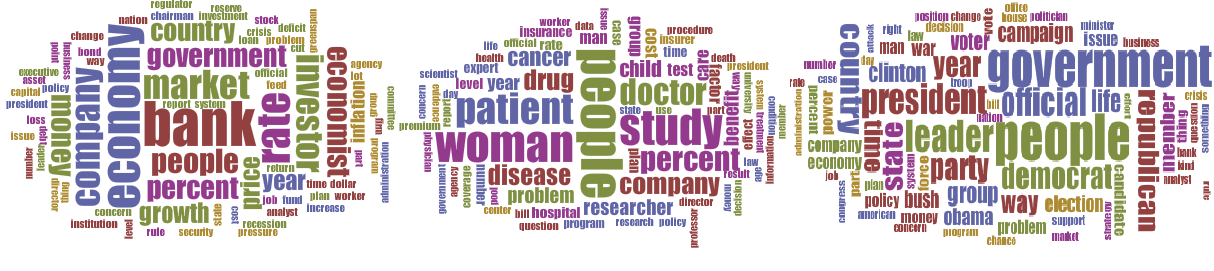
\includegraphics[width=0.70\textwidth]{../images/clouds.png}}
            \caption{Key participants in the \emph{Economics}, \emph{Health} and \emph{Politics} subcorpora}
            \label{fig:clouds}
            \end{figure}


            \begin{figure}[htb!]
            \centering
            \addvbuffer[12pt 8pt]{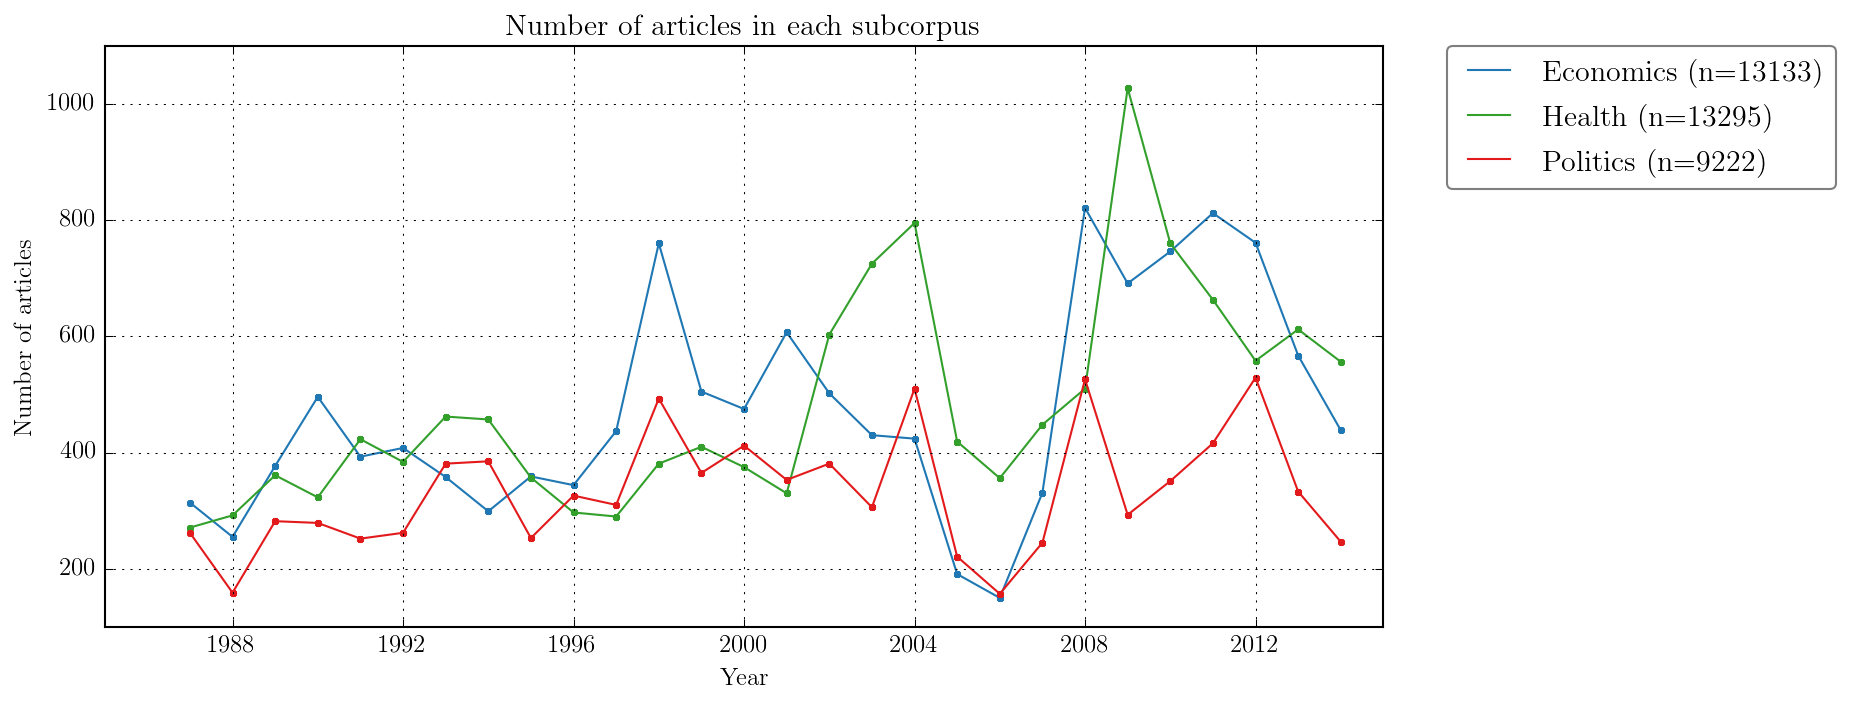
\includegraphics[width=.70\textwidth]{../images/number-of-articles-in-each-subcorpus.png}}
            \caption{Number of articles in each subcorpus}
            \label{fig:echepol_riskwords}
            \end{figure}

            \begin{figure}[htb!]
            \centering
            \addvbuffer[12pt 8pt]{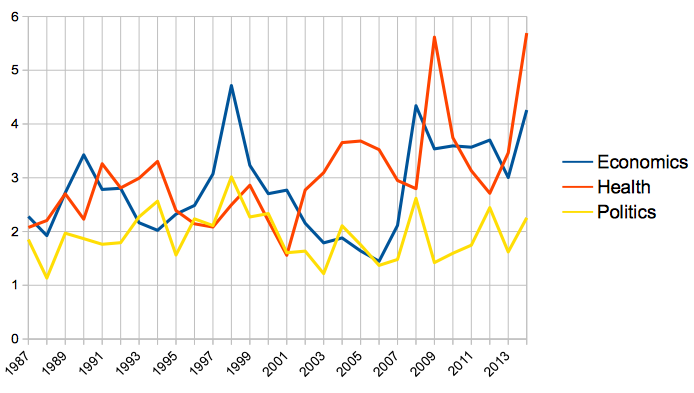
\includegraphics[width=.70\textwidth]{../images/echepol_riskwords.png}}
            \caption{Risk words per total number of article topics per year}
            \label{fig:echepol_riskwords}
            \end{figure}
            %
            %Due to time constraints, we restricted the topic comparison to domains that had yielded interesting insights in the earlier interrogations. Further, we found that the smaller size of the subcorpora limited us to lexicogrammatical queries that outputted a large enough number of results for quantitative reliability. Thus, we focussed on the following three areas:

             \begin{table}[htb!]
             \centering
             \small
             \begin{tabular}{|l|l|l|}
                          \hline
                          \textbf{Economics}   & \textbf{Health}         & \textbf{Politics}     \\ \hline
                          political   & high           & political    \\ \hline
                          big         & great          & great        \\ \hline
                          economic    & low            & big          \\ \hline
                          financial   & other          & high         \\ \hline
                          great       & serious        & own          \\ \hline
                          high        & financial      & serious      \\ \hline
                          more        & potential      & new          \\ \hline
                          real        & medical        & real         \\ \hline
                          systemic    & more           & considerable \\ \hline
                          significant & significant    & more         \\ \hline
                          new         & cardiovascular & other        \\ \hline
                          little      & political      & significant  \\ \hline
                          global      & possible       & economic     \\ \hline
                          serious     & small          & financial    \\ \hline
                          other       & real           & potential    \\ \hline
                          excessive   & such           & personal     \\ \hline
                          potential   & genetic        & little       \\ \hline
                          such        & ovarian        & such         \\ \hline
                          much        & same           & public       \\ \hline
                          own         & bad            & military     \\ \hline
                          \end{tabular}
                          \caption{Most common adjectives modifying nominal risks in the topic subcorpora}
                          \label{tab:echepo_adjmod}
             \end{table}

\section{Health}

    Our topic subcorpora were much smaller than our main corpus. As a result, lexicogrammatical querying did not yield quantitatively reliable results. Accordingly, other kinds of corpus linguistic investigation, not reliant on grammatical structure, were applied. 

    First, we considered \emph{keywords}---that is, words that were unusually frequent within the health corpus when compared to the corpus as as a whole.

    Linear regression was used to determine the slope of each keyword's trajectory, and ensure that the p-value of this slope was below 0.05. Results were then sorted into two groups, based on the incline\slash decline of the slope.

    \begin{figure}[htb!]
    \centering
    \begin{minipage}{.48\textwidth}
    \centering
    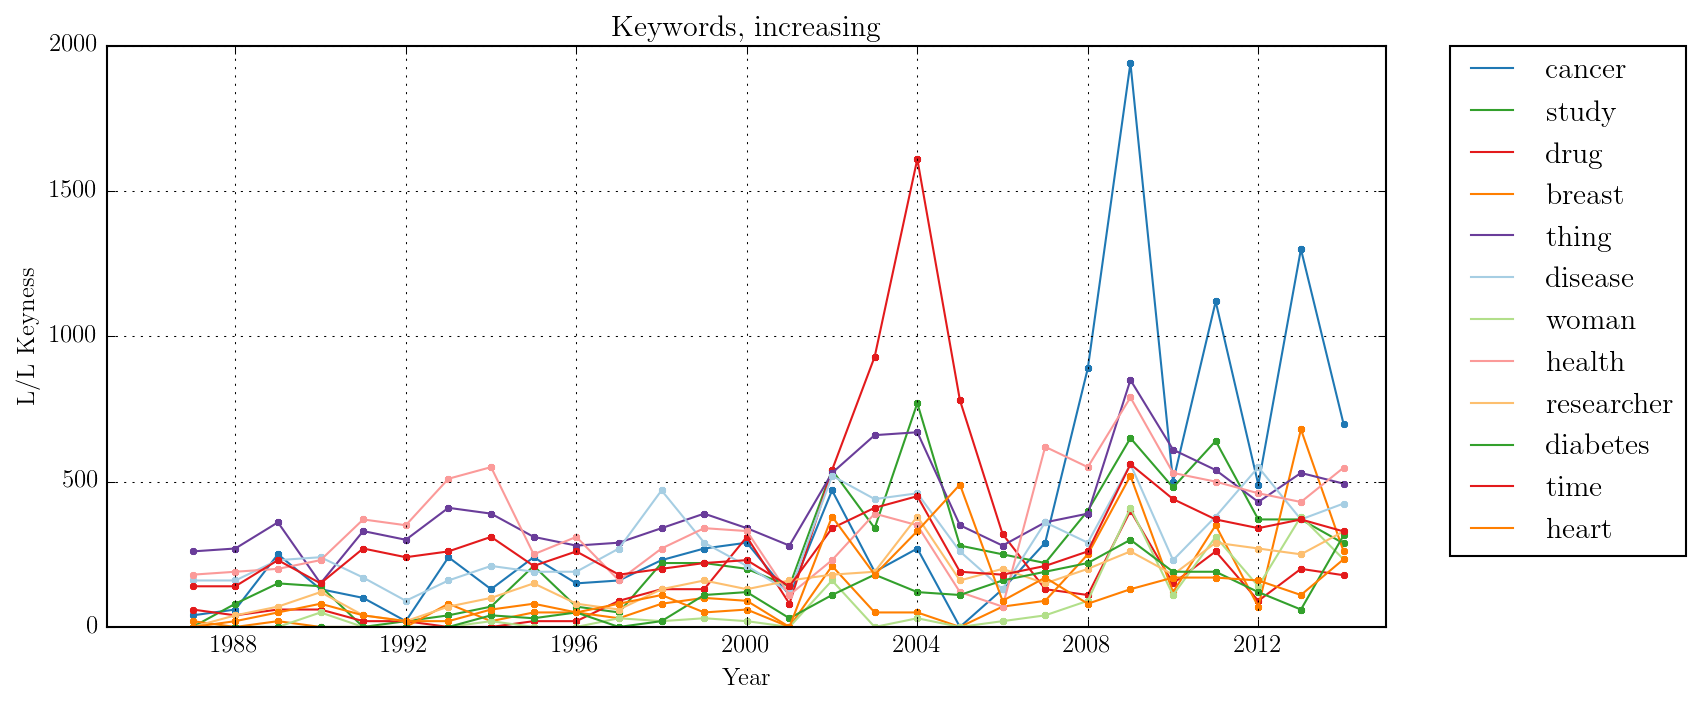
\includegraphics[width=.95\textwidth]{../images/keywords-increasing.png}
    \caption{Keywords becoming more key over time}
    \label{fig:key-inc}
    \end{minipage}%
    \begin{minipage}{.48\textwidth}
    \centering
    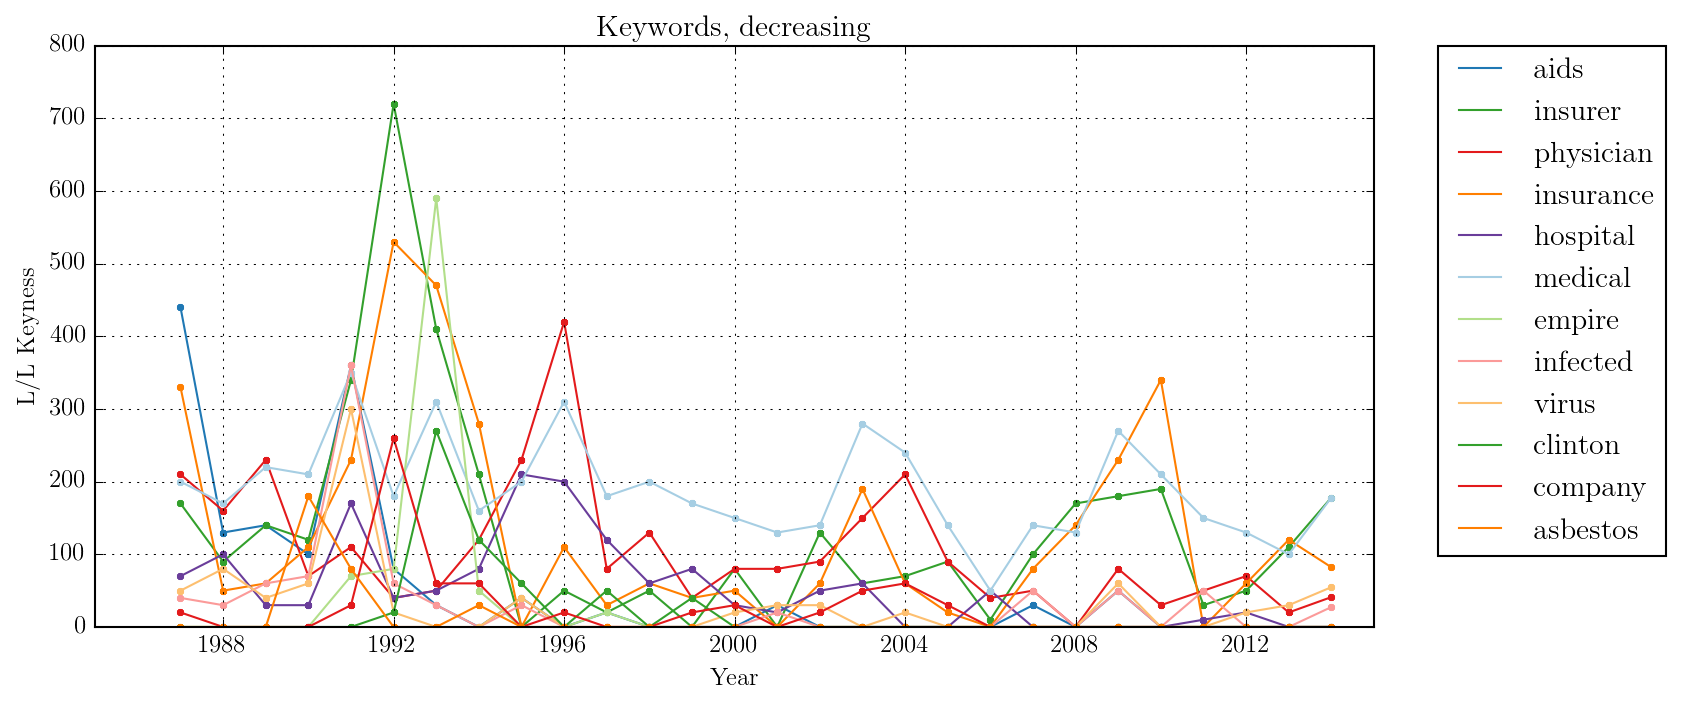
\includegraphics[width=.95\textwidth]{../images/keywords-decreasing.png}
    \caption{Keywords becoming less key over time}
    \label{fig:key-dec}
    \end{minipage}
    \end{figure}

    Next, we were interested in \emph{bigrams}---that is, words that occur beside each other multiple times within a corpus. Bigrams containing a stopword were excluded from analysis, as these results were generally common clusters of closed class words (\emph{in the}, \emph{of a}, \emph{one day}, etc.). Again, linear regression was used to group results into increasing and decreasing groups.

    \noindent
    \begin{figure}[htb!]
    \centering
    \begin{minipage}{.48\textwidth}
    \centering
    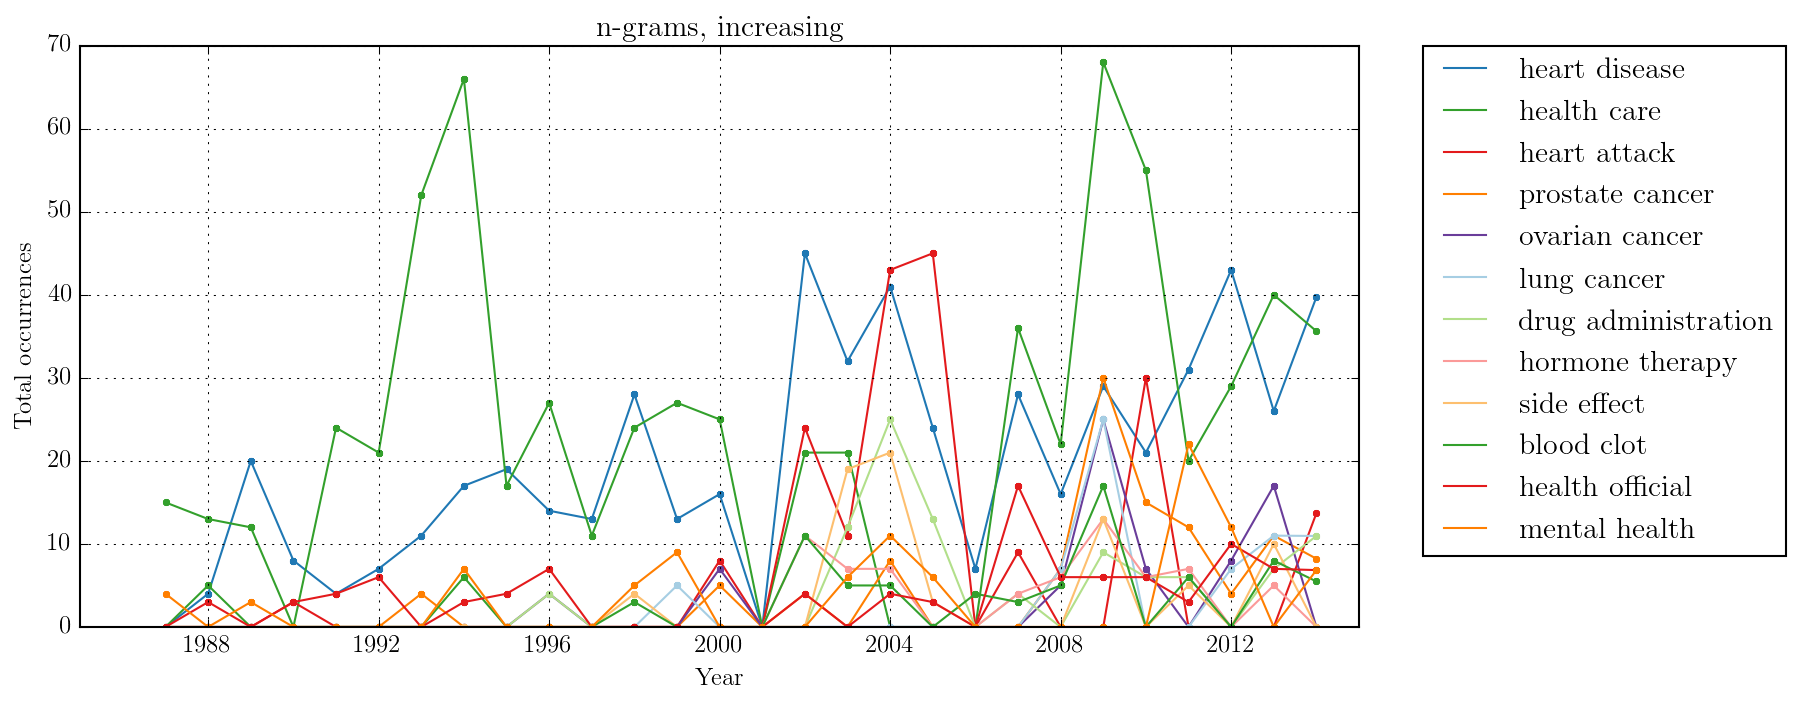
\includegraphics[width=.95\textwidth]{../images/ngrams-increasing.png}
    \caption{bi-grams becoming more frequent over time}
    \label{fig:ngram-inc}
    \end{minipage}%
    \begin{minipage}{.48\textwidth}
    \centering
    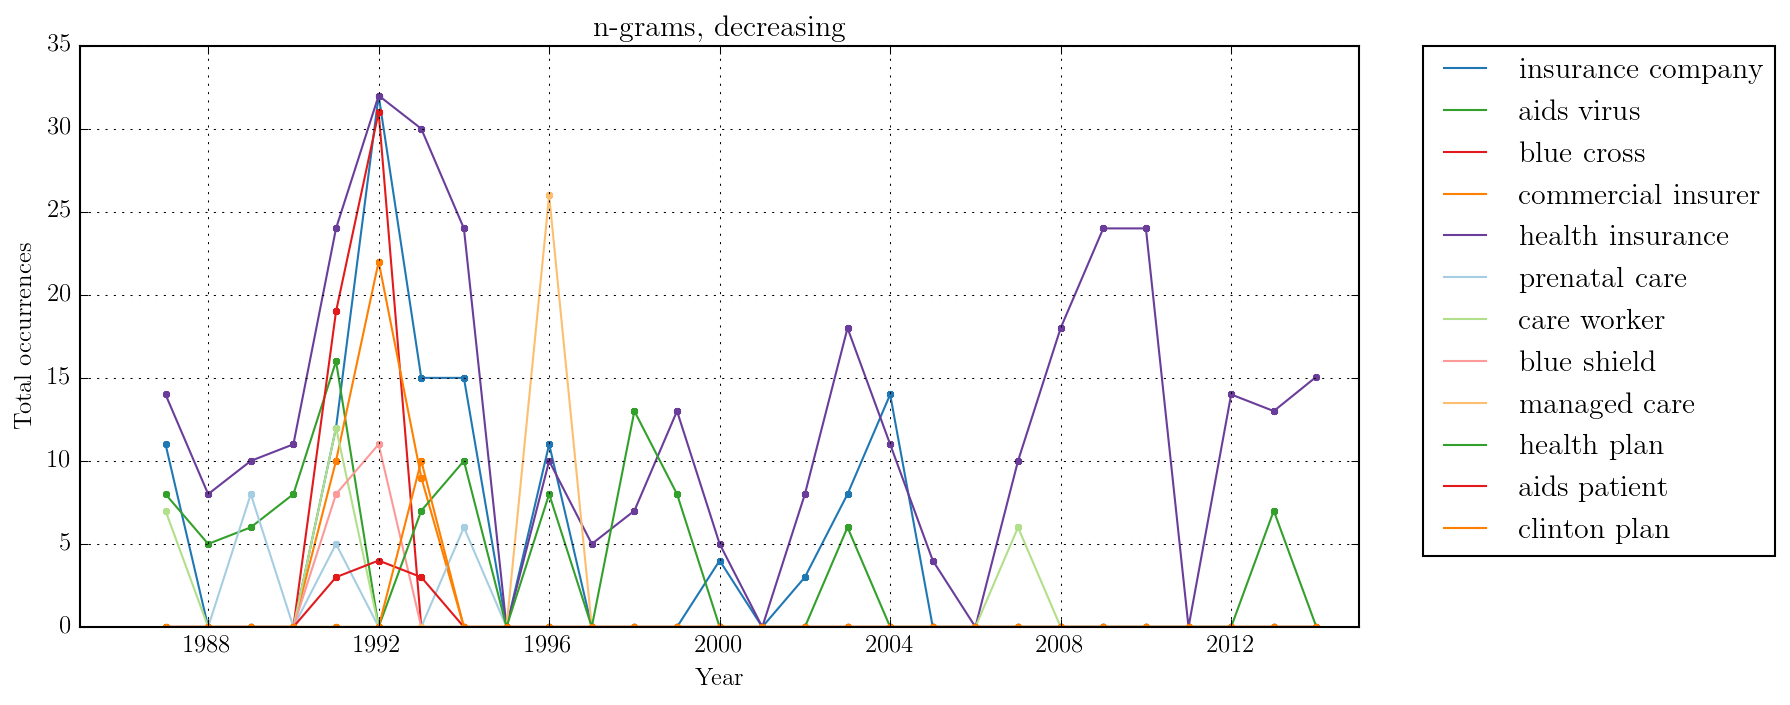
\includegraphics[width=.95\textwidth]{../images/ngrams-decreasing.png}
    \caption{bi-grams becoming less frequent over time}
    \label{fig:ngram-dec}
    \end{minipage}
    \end{figure}

We grouped these into themes, with results entered into one or more categories. Ambiguous results were often concordanced in order to determine the main context of use: \emph{athlete}, for example, could indicate the health condition (\emph{Athlete's foot}), a chain of footwear stores, or denote athletes themselves. The latter was revealed to be by far the most common context, and athlete was thus added to \emph{People, everyday}.

\subsection{Nominal groups in the health subcorpus}

The final part of our investigation of the health subcorpus looked at key nouns or nominal groups. By measuring the slope of trend lines, we could ascertain which groups were becoming more or less common.

    \noindent
    \begin{figure}[htb!]
    \centering
    \begin{minipage}{.48\textwidth}
    \centering
    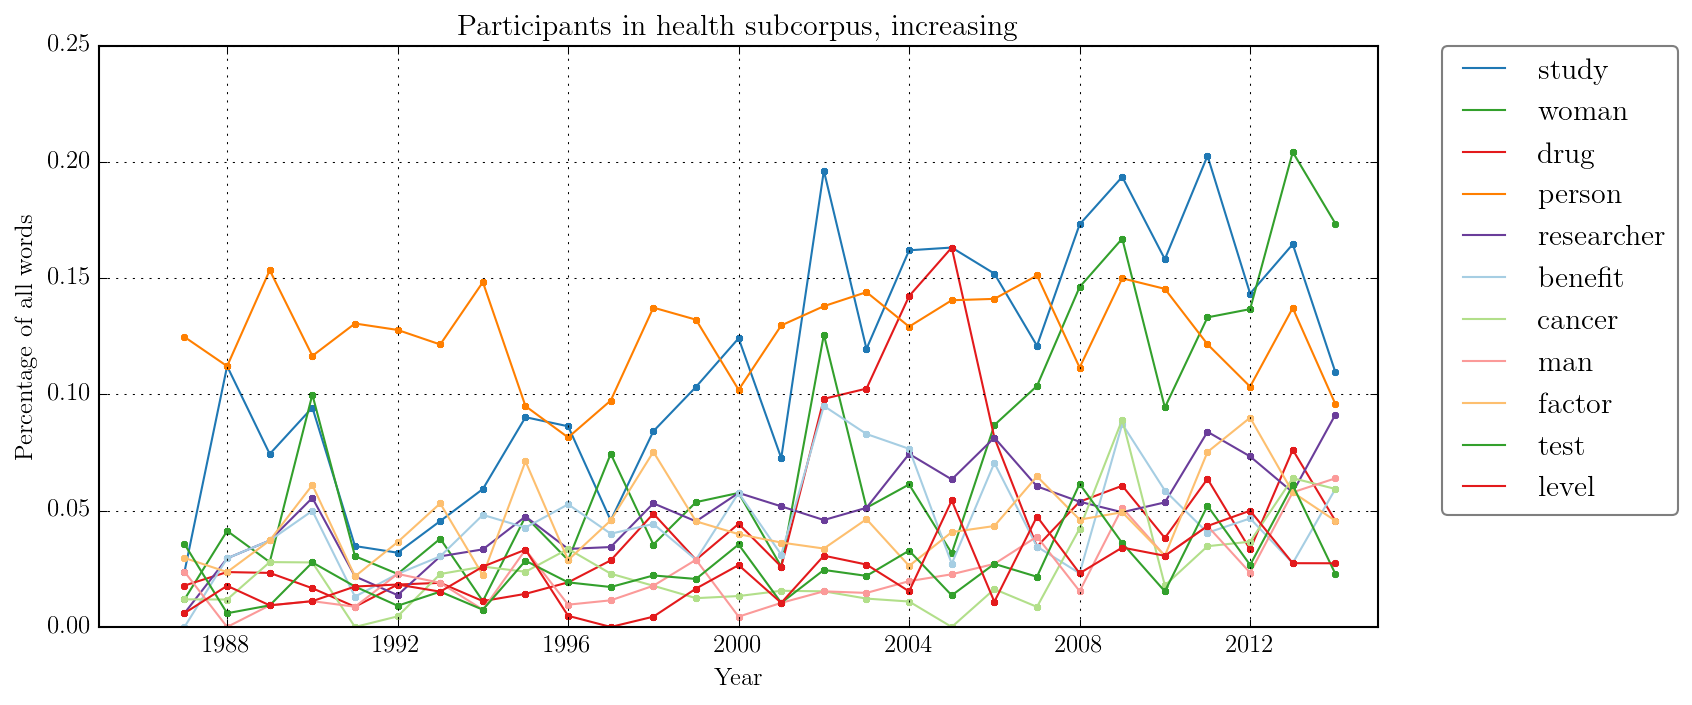
\includegraphics[width=.95\textwidth]{../images/1.png}
    \caption{Absolute frequency of nominal groups becoming more frequent over time}
    \label{fig:1}
    \end{minipage}%
    \begin{minipage}{.48\textwidth}
    \centering
    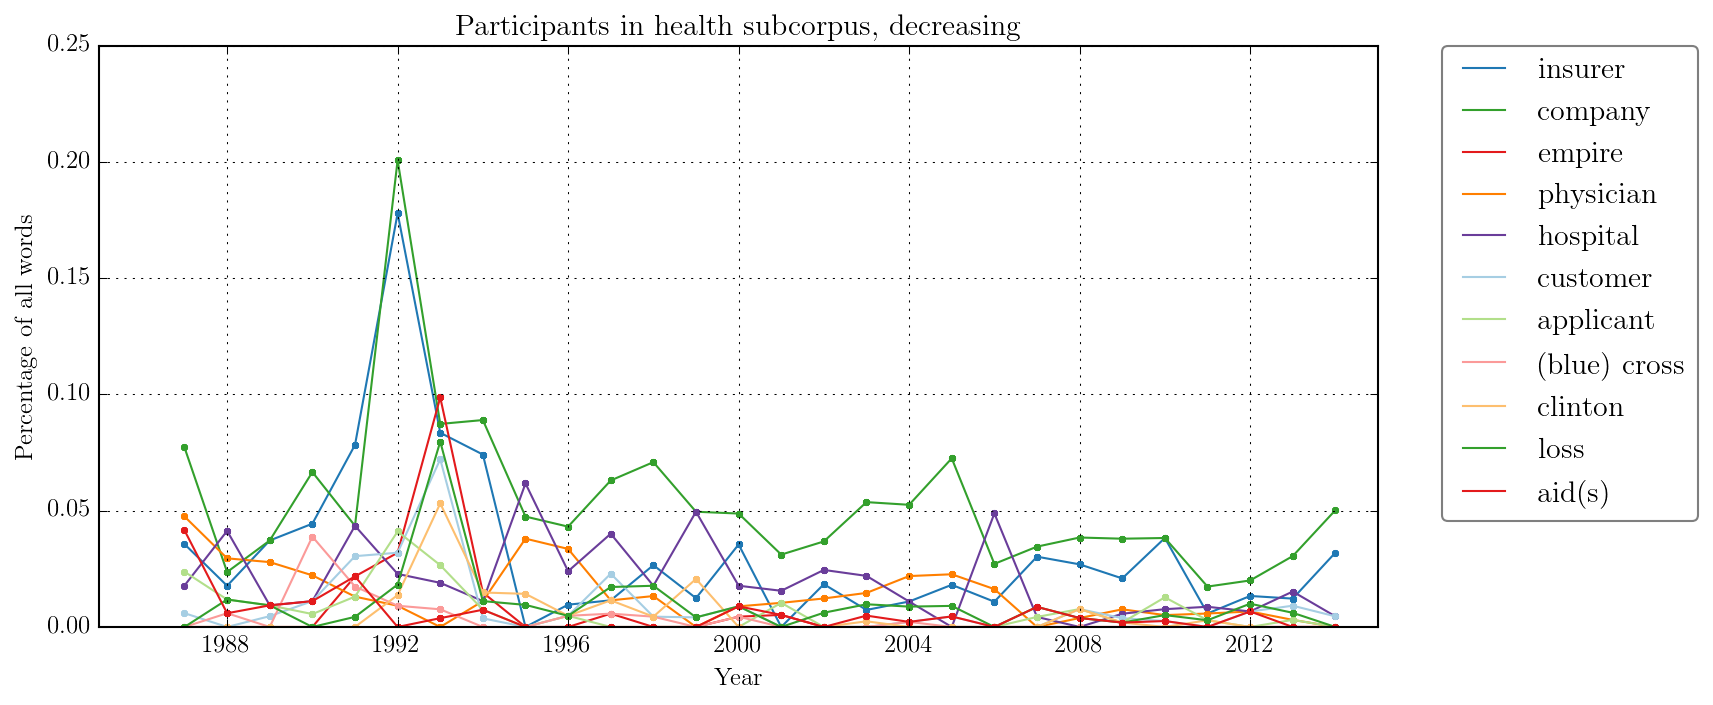
\includegraphics[width=.95\textwidth]{../images/2.png}
    \caption{Relative frequency of nominal groups becoming more frequent over time}
    \label{fig:2}
    \end{minipage}
    \end{figure}
    \noindent
    \begin{figure}[htb!]
    \centering
    \begin{minipage}{.48\textwidth}
    \centering
    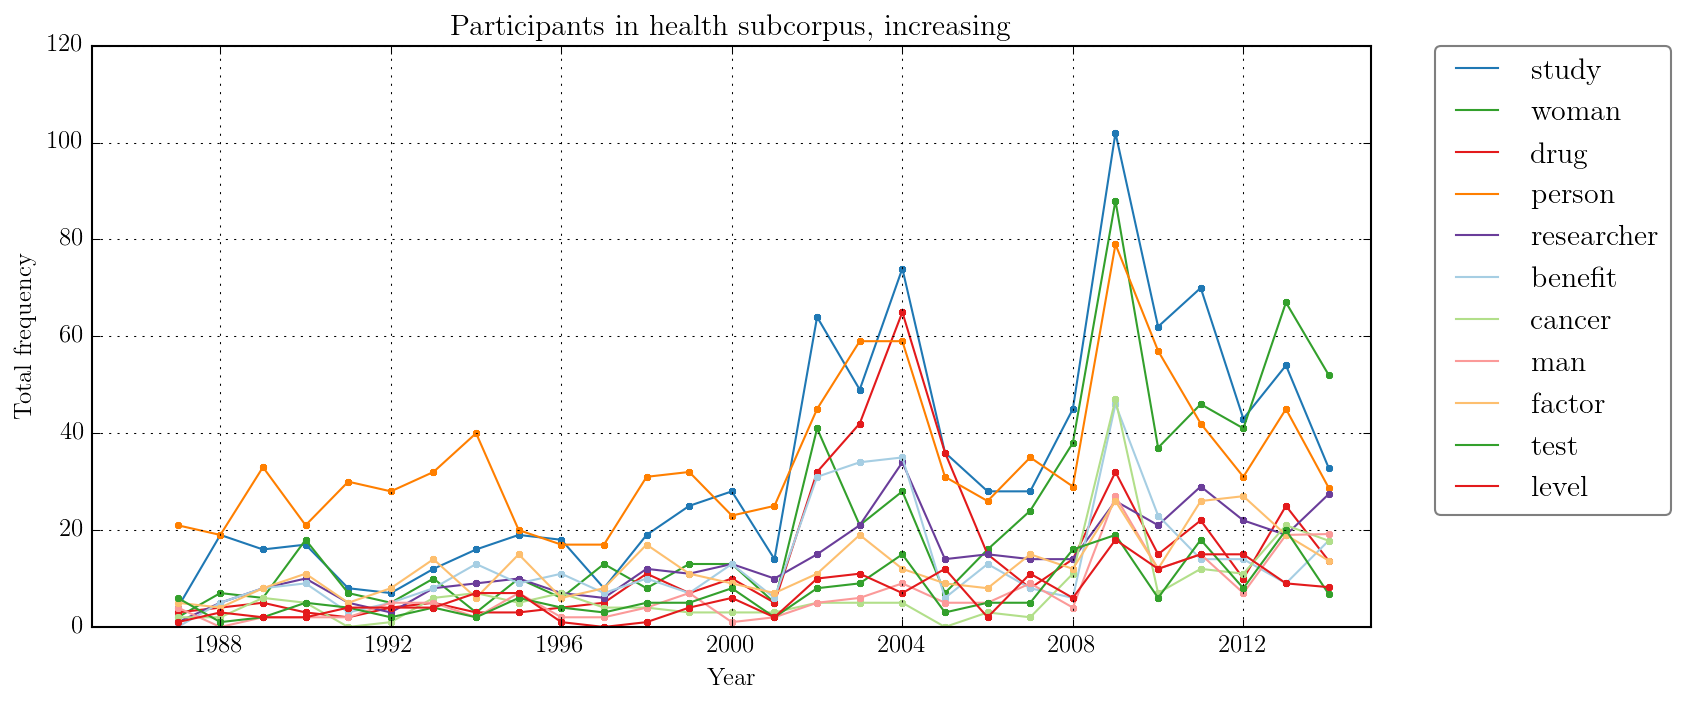
\includegraphics[width=.95\textwidth]{../images/3.png}
    \caption{Relative frequency of nominal groups becoming more frequent over time}
    \label{fig:3}
    \end{minipage}%
    \begin{minipage}{.48\textwidth}
    \centering
    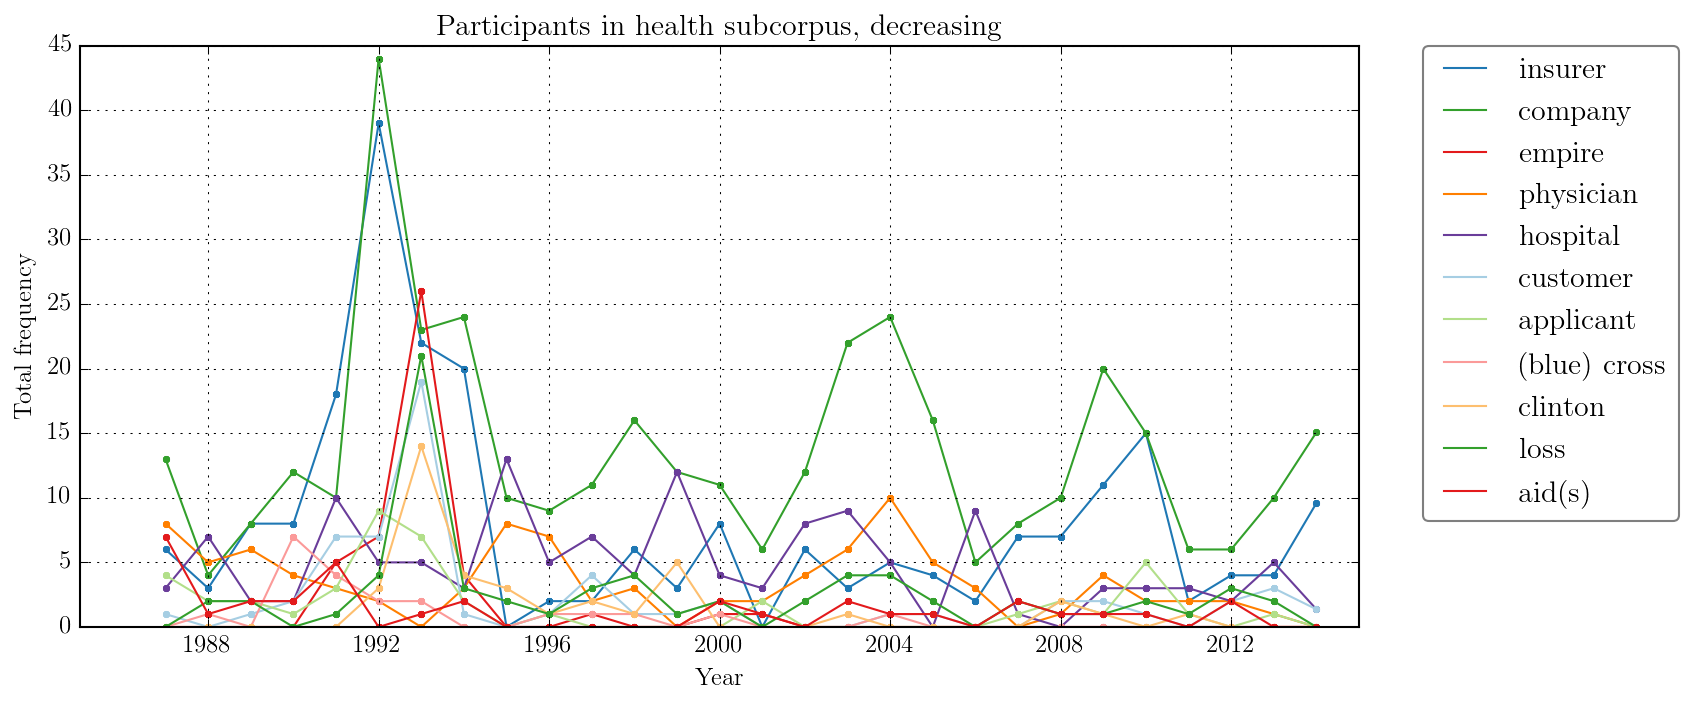
\includegraphics[width=.95\textwidth]{../images/4.png}
    \caption{Relative frequency of nominal groups becoming less frequent over time}
    \label{fig:4}
    \end{minipage}
    \end{figure}

The first major theme that emerges from this interrogation is the shift from infectious to non-infectious disease.

A second point of interest is the decline in terms related to insurance.

Though the prevalence of health insurance in mid 1990s articles was unexpected, as it corresponds with Hillary Clinton's efforts to increase health insurance coverage in the USA, unexpected was the lack of an upswing in insurance terms during the pushes for healthcare reform throughout the Obama administration.



Given the continuing disc
Also apparent is an upward trend for nominal groups related to research (\emph{study, percent, research, etc.}).

This finding was of particular interest, given that the increasing contestation of academic and scientific research are core hypotheses made by Beck.

Concordancing was used to look for evidence of contestation when the nominal groups related to research were instantiated.



\section{Summary}

Broadly speaking, institutional social actors, political representatives and the like appear to have been displaced by individual human actors and components within their everyday life world.

The exception to this rule is research, which

Though further investigation into the emergence of research as a key semantic domain within risk discourse is needed, we hypothesise that it

The increasing commonality of data journalism, where journalists may conduct

Another potential factor is that the exponential increase in academic publications, as well as the increasing ease of access (via the web) has made reporting of 

This may also be a part of the increase in health risk discourse as well.

The lack of contestation points to an area in which Beck's conceptualisation of risk in late modernity may be at odds




\section{Issues in the health corpus investigation}

The first major issue was the smaller size of the corpus, which necessitated different kinds of analysis.

Within keywording and ngramming, it became clear that broader linguistic change and specific events are difficult to separate.

This, however, is where we can see the clearest examples of the link between events and language change. Interspersed throughout the keywords and n-grams are terms ranging in specificity. It is through categorisation of these varying levels that we can smooth out the 

The keywording in particular revealed a number of ambiguities. A more reliable\slash systematic method for grouping keywords would ameliorate this concern.

\section{Summary}

    The smaller size of topic subcorpora necessitated different kinds of analysis. Fortunately, such methods are well documented within corpus assisted discourse studies. Following on from these methodologies, we located particularly frequent terms, and analysed them in their context of use.

    % analysis here

    Ultimately, the ways in which a corpus can be analysed are dependent on the size of the corpus. 



